\q{14}{I'll Take Civic Participation for 100 Points Please}
\vskip 0.1 in
A Berkeley political science professor is concerned about their students' knowledge of current U.S political events. To assess their civic participation, the professor sent a survey to 150 randomly-selected students quizzing them on their knowledge of recent news out of a total score of 100. In the 150-student sample, the mean score was 71.7 and standard deviation was 6.2. Here is a plot of the distribution of the 150 scores:

\begin{center}
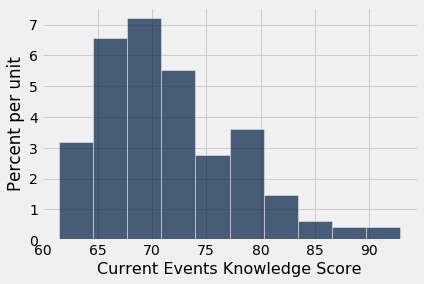
\includegraphics[scale=.7]{figures/civic_hist.png}
\end{center}

\textbf{For parts a - c, choose the option that best completes the blank.}
\vskip .1in
\begin{enumerate}
\subq{2} This distribution is \lsi++\bk++.
\vskip 0.1in
	\bubble \quad Left skewed\newline
	\solutionbubble \quad Right skewed\newline
	\bubble \quad Normally distributed
\vskip 0.2in
\subq{2} The mean of the above histogram is \lsi++\bk++ the median.
\vskip 0.1in
	\solutionbubble \quad higher than\newline
	\bubble \quad lower than\newline
	\bubble \quad equal to

\vskip 0.2in
\subq{2} The professor can expect at least \lsi++\bkshort++ of the scores to be between 59.3 and 84.1. 
\vskip 0.1in
	\bubble \quad 95\%\newline
	\bubble \quad 89\%\newline
	\solutionbubble \quad 75\%\newline
	\bubble \quad We don't have enough information to tell.
\clearpage
Although the professor only ended up with 150 entries for the survey, the professor decided to assume that this distribution of survey scores is representative of the entire  UC Berkeley student population. To get a better estimate of the entire student population’s knowledge, the professor conducts the following analysis:
\vskip 0.1in
\begin{itemize}
\item The professor resamples 150 scores with replacement from the original survey distribution.
\item The professor calculate the average of those 150 scores and store it in an array called \lsi+scores+. 
\item The professor repeat the above process 10,000 times.
\end{itemize}
\vskip 0.1in
Thus, \lsi+scores+ is an array of 10,000 average survey scores.
\vskip 0.2in
\subq{2} If the professor graphed the \lsi+scores+ distribution as a histogram, what would the shape of the histogram look like?
\vskip 0.1in
\begin{tabular}{l@{\hskip 1in}l@{\hskip 1in}l@{\hskip 1in}l}
\bubble \quad Left skewed
&\bubble \quad Right skewed\\[6pt]
\solutionbubble \quad Normally distributed
&\bubble \quad We don't have enough information to tell.
\end{tabular}

\vskip 0.2in
\subq{2} If the professor graphed the \lsi+scores+ distribution as a histogram, which of the following would be the best approximation of the mean/center of the distribution?
\vskip 0.1in
\begin{tabular}{l@{\hskip 1in}l@{\hskip 1in}l@{\hskip 1in}l}
\bubble \quad 7.17
 &\solutionbubble \quad 71.7  \\[6pt]
\bubble \quad 50
&\bubble \quad We don't have enough information to tell.
\end{tabular}

\vskip 0.22in
\subq{2} If the professor graphed the \lsi+scores+ distribution as a histogram, which of the following is the best approximation for the standard deviation of the distribution?
\vskip 0.1in
\begin{tabular}{l@{\hskip 1in}l@{\hskip 1in}l@{\hskip 1in}l}
\bubble \quad 6.2
&\solutionbubble \quad ${\displaystyle \frac{6.2}{\sqrt{150}} }$\\[6pt]
\bubble \quad ${\displaystyle \frac{\sqrt{150}}{6.2}}$
&\bubble \quad We don't have enough information to tell.
\end{tabular}

\vskip 0.2in
\subq{2} Still looking at the \lsi+scores+ distribution (i.e. the distribution of average survey scores), if we take only the average scores that are 1 SD of sample means away from the true average, roughly how much of the data (average survey scores) would we be looking at? 
\vskip 0.1in
\begin{tabular}{l@{\hskip 1in}l@{\hskip 1in}l@{\hskip 1in}l}
\bubble \quad 10\%
&\solutionbubble \quad 68\%\\[10pt]
\bubble \quad 75\%
&\bubble \quad 95\%
\end{tabular}
\end{enumerate}